\graphicspath{{\currfiledir/images/}}

%----------------------------------------------------------------------------------------
%	Resultados
%----------------------------------------------------------------------------------------
\chapter{Resultados}
O trabalho foi desenvolvido em \emph{Python 3}, com uso da biblioteca \emph{NetworkX} \cite{networkx2021}.

Para a execução dos testes, foram selecionados três grafos, sendo deles um grafo simples, utilizado para visualização exata dos valores de centralidade para cada caminho mínimo. Os demais dois grafos são modelos da vida real dados pelas aplicações do clube de karatê de Zachary e a rede de jogos de futebol americano. Buscou-se selecionar redes que contivessem número de vértices e arestas distintas, para que fosse possível obter resultados não viciados em relação ao tamanho do grafo sobre os quais seriam executados os testes. Dito isso, os grafos selecionadas representam diferentes tipos de redes e possuem quantidades de vértices que variam de 5 a 115. A Tabela~\ref{sec5:tab_grafos_teste} apresenta a descrição das redes nas quais foram executados os testes propostos.

\begin{table}[!htp]
	\centering
	\caption{Detalhamento das redes selecionadas.}
	\label{sec5:tab_grafos_teste}
	\begin{tabular}{|c|c|c|c|c|}
		\hline
		\textbf{Rede} & \textbf{Vértices} & \textbf{Arestas} & \textbf{Tipo}   & \textbf{Classificação} \\ \hline
		Simple        & 5                 & 6                & Não direcionado & Teste                  \\
		Zachary       & 34                & 78               & Não direcionado & Social                 \\
		Football      & 115               & 613              & Não direcionado & Informação             \\ \hline
	\end{tabular}
\end{table}

A Tabela~\ref{sec5:centralidade_grafo_teste} representa os valores de centralidade calculados pelo Algoritmo~\ref{sec4:funcao_simple_graph_generator} para o grafo mais simples. A ordem apresentada na tabela depende do contexto de análise. Para este grafo, foi feita a ordenação de tal forma a agrupar ou deixar mais próximos os vértices iguais. Por exemplo, as primeiras linhas desta tabela estão ordenadas primeiro com todos os caminhos mínimos que iniciam no vértice 1 e assim por diante.

\begin{table}[!htp]
	\centering
	\caption{Valores de centralidade do grafo simples, Algoritmo~\ref{sec4:funcao_simple_graph_generator}.}
	\label{sec5:centralidade_grafo_teste}
	\resizebox{3cm}{!}{
		\begin{tabular}{|c|c|}
			\hline
			\textbf{Path} & \textbf{Centrality}	\\ \hline
			{[}1, 2{]}    & {[}0.050{]}			\\
			{[}1, 3{]}    & {[}0.075{]}			\\
			{[}1, 5{]}    & {[}0.075{]}			\\
			{[}1, 3, 4{]} & {[}0.016{]} 		\\
			{[}2, 1{]}    & {[}0.050{]}			\\
			{[}2, 3{]}    & {[}0.050{]}			\\
			{[}2, 1, 5{]} & {[}0.016{]} 		\\
			{[}2, 3, 4{]} & {[}0.016{]} 		\\
			{[}3, 1{]}    & {[}0.075{]}			\\
			{[}3, 2{]}    & {[}0.050{]}			\\
			{[}3, 4{]}    & {[}0.075{]}			\\
			{[}3, 1, 5{]} & {[}0.016{]}			\\
			{[}5, 1{]}    & {[}0.075{]}			\\
			{[}5, 4{]}    & {[}0.025{]}			\\
			{[}5, 1, 2{]} & {[}0.016{]} 		\\
			{[}5, 1, 3{]} & {[}0.016{]} 		\\
			{[}4, 3{]}    & {[}0.075{]}			\\
			{[}4, 5{]}    & {[}0.025{]}			\\
			{[}4, 3, 1{]} & {[}0.016{]} 		\\
			{[}4, 3, 2{]} & {[}0.016{]} 		\\ \hline
		\end{tabular}
	}
\end{table}

\newpage

Para os grafos do clube de karatê de Zachary e da rede de jogos de futebol americano, os resultados foram apresentados em gráficos, pois suas tabelas são extensas. Serão apresentados dois tipos de gráficos, um com os valores de centralidade dos camino mínimos normalizados e outro com os valores de centralidade não normalizados e na escala logarítmica.

O Gráfico~\ref{sec5:short_path_centrality_ex2} e o Gráfico~\ref{sec5:short_path_centrality_ex3} distribuem os valores de centralidade, normalizados, dos caminhos mínimos no eixo $y$, de forma ordenada (crescente), enquanto o eixo $x$ representa os caminhos mínimos rotulados sequencialmente. Nesta visualização o percurso exato de cada um dos caminhos mínimos não nos interessa.

\begin{figure}[!htb]
    \centering
    \begin{subfigure}{.5\textwidth}
        \centering
        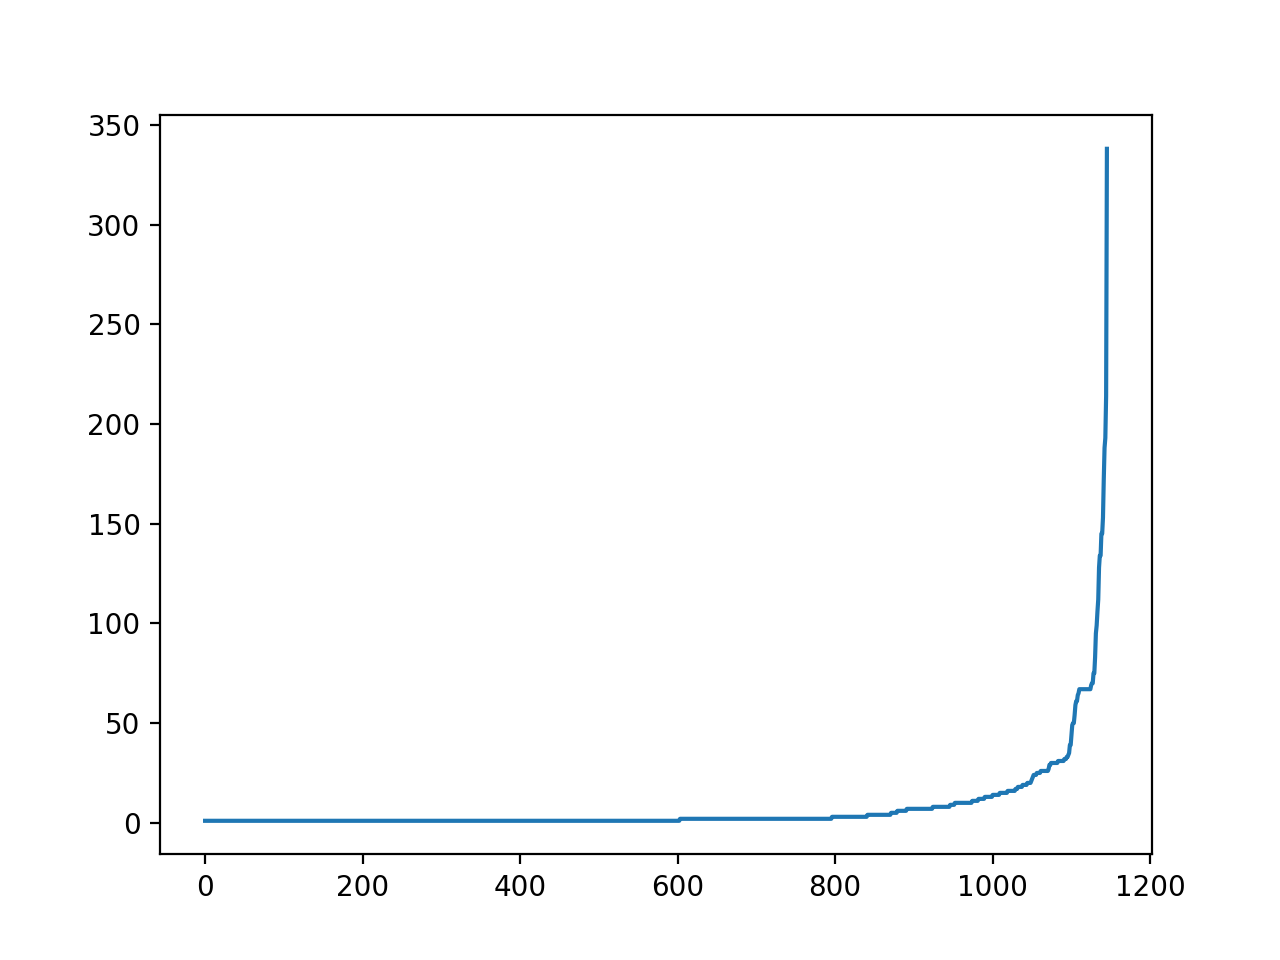
\includegraphics[scale=0.5]{short_path_centrality_ex2.png}
        \caption{Clube de karatê de Zachary.}
        \label{sec5:short_path_centrality_ex2}
    \end{subfigure}%
    \begin{subfigure}{.5\textwidth}
        \centering
        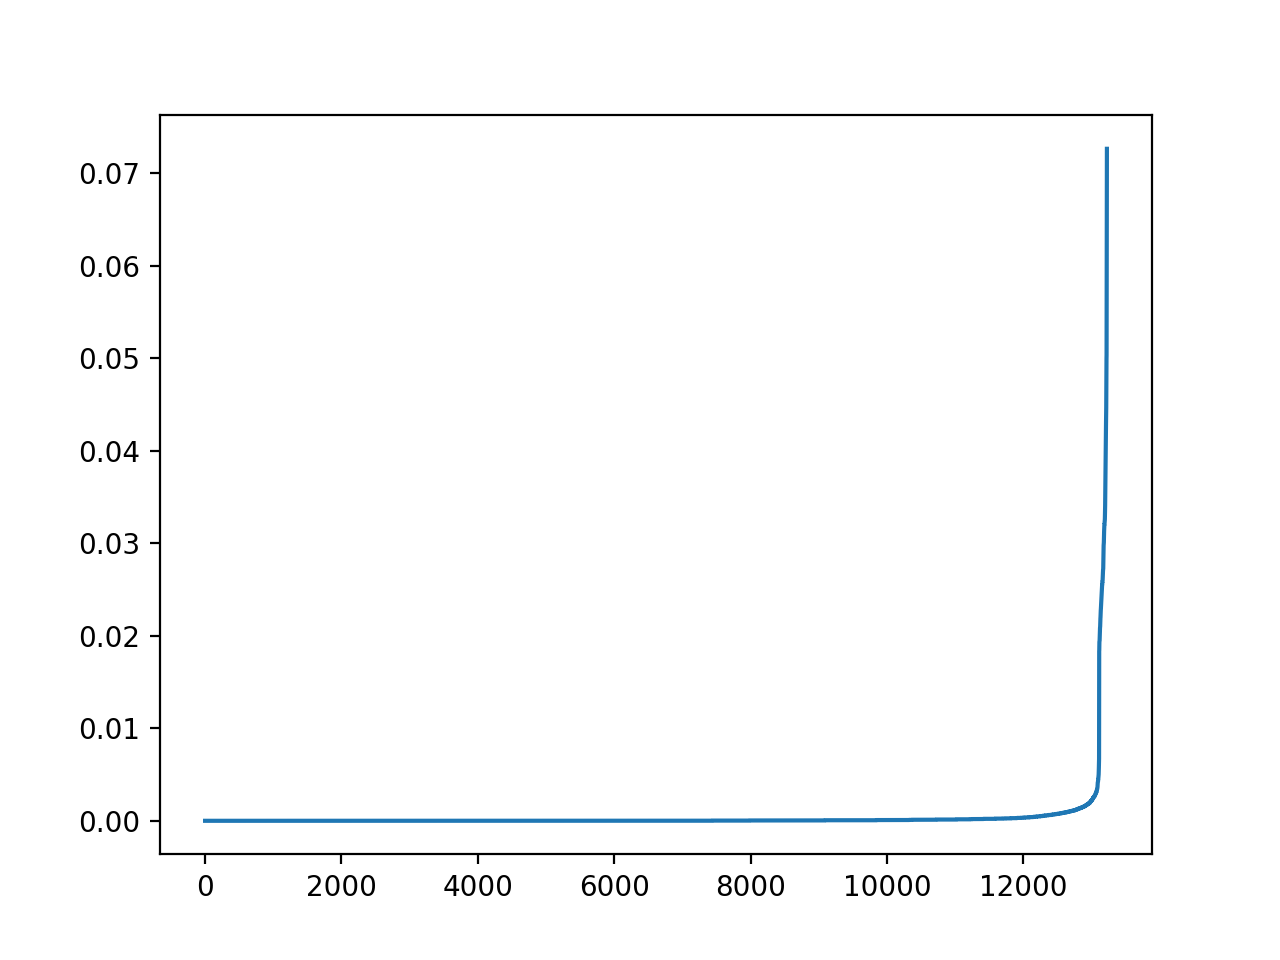
\includegraphics[scale=0.5]{short_path_centrality_ex3.png}
        \caption{Rede de jogos de futebol americano.}
        \label{sec5:short_path_centrality_ex3}
    \end{subfigure}
    \caption{Distribuição dos valores de centralidade, normalizados, dos caminhos mínimos.}
    \label{sec5:grafico_centralidade_normalizados}
\end{figure}

O Gráfico~\ref{sec5:short_path_centrality_ex2_log} e o Gráfico~\ref{sec5:short_path_centrality_ex3_log} distribuem os valores de centralidade, não normalizados e na escala logarítmica, dos caminhos mínimos no eixo $y$, de forma ordenada (crescente).

\begin{figure}[!htb]
    \centering
    \begin{subfigure}{.5\textwidth}
        \centering
        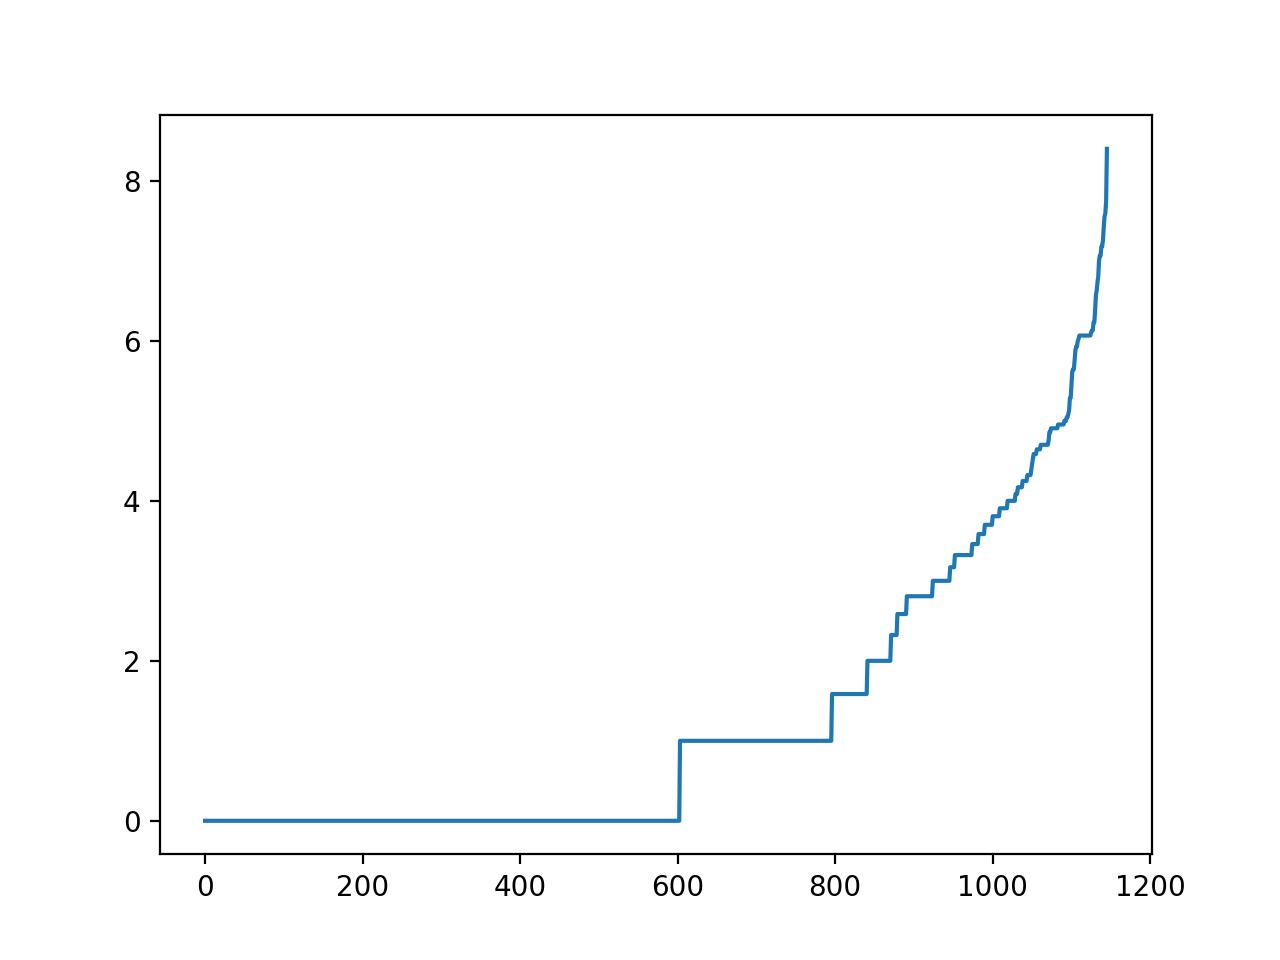
\includegraphics[scale=0.5]{short_path_centrality_ex2_log.png}
        \caption{Clube de karatê de Zachary.}
        \label{sec5:short_path_centrality_ex2_log}
    \end{subfigure}%
    \begin{subfigure}{.5\textwidth}
        \centering
        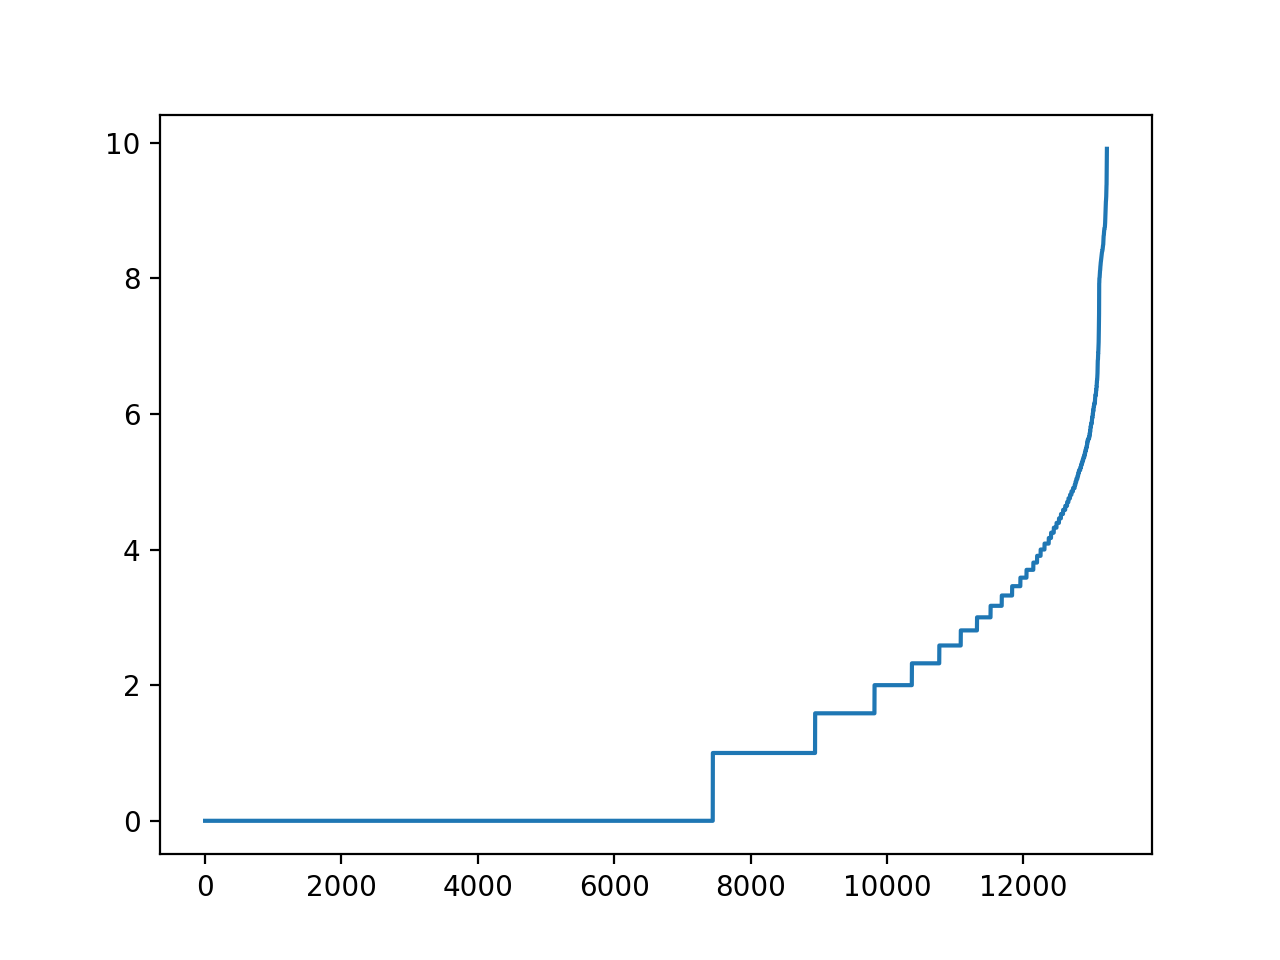
\includegraphics[scale=0.5]{short_path_centrality_ex3_log.png}
        \caption{Rede de jogos de futebol americano.}
        \label{sec5:short_path_centrality_ex3_log}
    \end{subfigure}
    \caption{Distribuição dos valores de centralidade, não normalizados e na escala logarítmica, dos caminhos mínimos.}
    \label{sec5:grafico_centralidade_normalizados}
\end{figure}